\documentclass[12pt]{article}
\usepackage[utf8]{inputenc}

%%% PAGE DIMENSIONS
\usepackage{geometry} % to change the page dimensions
\geometry{margin=0.5in}

\usepackage{graphicx} 

%%% PACKAGES
\usepackage{booktabs} 
\usepackage{array} 
\usepackage{paralist}
\usepackage{verbatim} 
\usepackage{subfig} 
\usepackage{longtable}
\usepackage{listings}
\usepackage{amsmath}
\usepackage{pdfpages}


%%% HEADERS & FOOTERS
\usepackage{fancyhdr}
\pagestyle{fancy} 
\renewcommand{\headrulewidth}{0pt} 
\lhead{}\chead{}\rhead{}
\lfoot{}\cfoot{\thepage}\rfoot{}

%%% TABLE FONT
\usepackage{etoolbox}
\AtBeginEnvironment{longtable}{\sffamily}
\AtBeginEnvironment{table}{\sffamily}

%%% CODE FONT
\newcommand{\code}[1]{\texttt{#1}}

%%% SECTION TITLE APPEARANCE
\usepackage{sectsty}
\allsectionsfont{\sffamily\mdseries\upshape} 

%%%
\title{ATSC 507 - HW1}
\author{Eve Wicksteed}
\date{January 2020}

\begin{document}

\maketitle

\section*{Part 1}

The following graph shows the altitude of the ground and the altitudes of the following isobaric surfaces: 100, 90, 80, 70, 60, 50, 40, 30, 20, 10, 5, 2 kPa.
Altitudes were calculated using the hypsometric equation:

$$
P_{2}=P_{1} \cdot \exp \left(\frac{z_{1}-z_{2}}{a \cdot \overline{T_{v}}}\right)
$$


\graphicspath{ {/Users/ewicksteed/Documents/Eve/507/HW1/} }

\begin{figure}[h]
    \centering
    \includegraphics[width=\textwidth]{200117part1_plot.png}
    \caption{x-z plot of altitudes and ground level}
    \label{fig:mesh1}
\end{figure}


\section*{Part 2}
Using the data from part 1, I interpolate pressure to ground level using the hypsometric equation. 
The table below shows the values of the x-domain, ground-level and surface pressure. 


\begin{longtable}{|l|l|l|}
\caption {Table of ground height and surface pressure for the x-domain} \\
    \hline
    \textbf{x (km)} & \textbf{z\_ground (km)} & \textbf{surface pressure (kPa)} \\ \hline
    \hline
    \endhead

    %
    0      & 0              & 95                     \\ \hline
    20     & 0              & 95.2                   \\ \hline
    40     & 0              & 95.4                   \\ \hline
    60     & 0              & 95.6                   \\ \hline
    80     & 0              & 95.8                   \\ \hline
    100    & 0              & 96                     \\ \hline
    120    & 0              & 96.2                   \\ \hline
    140    & 0              & 96.4                   \\ \hline
    160    & 0              & 96.6                   \\ \hline
    180    & 0              & 96.8                   \\ \hline
    200    & 0              & 97                     \\ \hline
    220    & 0              & 97.2                   \\ \hline
    240    & 0              & 97.4                   \\ \hline
    260    & 0.007885618    & 97.50810262            \\ \hline
    280    & 0.070224374    & 96.978406              \\ \hline
    300    & 0.190984253    & 95.76469456            \\ \hline
    320    & 0.362577482    & 93.96784119            \\ \hline
    340    & 0.574222245    & 91.73210462            \\ \hline
    360    & 0.812620145    & 89.228383              \\ \hline
    380    & 1.062791791    & 86.63658367            \\ \hline
    400    & 1.309018004    & 84.13009567            \\ \hline
    420    & 1.535827512    & 81.86428518            \\ \hline
    440    & 1.728969063    & 79.96962152            \\ \hline
    460    & 1.876306885    & 78.54890208            \\ \hline
    480    & 1.968583214    & 77.67732657            \\ \hline
    500    & 2              & 77.40391856            \\ \hline
    520    & 1.968583214    & 77.75291945            \\ \hline
    540    & 1.876306885    & 78.72415134            \\ \hline
    560    & 1.728969063    & 80.29185473            \\ \hline
    580    & 1.535827512    & 82.40208868            \\ \hline
    600    & 1.309018004    & 84.9693994             \\ \hline
    620    & 1.062791791    & 87.8740627             \\ \hline
    640    & 0.812620145    & 90.96167338            \\ \hline
    660    & 0.574222245    & 94.04700425            \\ \hline
    680    & 0.362577482    & 96.92367341            \\ \hline
    700    & 0.190984253    & 99.38010269            \\ \hline
    720    & 0.070224374    & 101.2206071            \\ \hline
    740    & 0.007885618    & 102.2886199            \\ \hline
    760    & 0              & 102.6                  \\ \hline
    780    & 0              & 102.8                  \\ \hline
    800    & 0              & 103                    \\ \hline
    820    & 0              & 103.2                  \\ \hline
    840    & 0              & 103.4                  \\ \hline
    860    & 0              & 103.6                  \\ \hline
    880    & 0              & 103.8                  \\ \hline
    900    & 0              & 104                    \\ \hline
    920    & 0              & 104.2                  \\ \hline
    940    & 0              & 104.4                  \\ \hline
    960    & 0              & 104.6                  \\ \hline
    980    & 0              & 104.8                  \\ \hline
    1000   & 0              & 105                    \\ \hline
    \end{longtable}

I also used \code{scipy.interpolate.interp1d} to calculate interpolated pressures at ground level 
(interpolated from sea-level pressure). The results from this method are almost the same as those from using the hypsometric
equation. A second table with two columns for pressure (one from \code{scipy.interpolate} and one from the 
hypsometric equation) can be found in Appendix 1.


\section*{Part 3}

Using the surface level pressure values calculated in Part 2, I plot the lines of constant $ \eta $ 
for $ \eta $ equal to the following values: 0, 0.1, 0.2, 0.3, 0.4, 0.5, 0.6, 0.7, 0.8, 0.85, 0.9, 0.95, 1.


\begin{figure}[h]
    \centering
    \includegraphics[width=\textwidth]{200117part3_plot2.png}
    \caption{x-p plot of pressure for constant $ \eta $}
    \label{fig:mesh1}
\end{figure}


\section*{Part 4}

Using the same $ \eta $ values as in Part 3, I plot the altiudes associated with constant $ \eta $.
To do this I used the hypsometric equation:
$$
z_{2}-z_{1} \approx a \cdot \bar{T}_{v} \cdot \ln \left(\frac{P_{1}}{P_{2}}\right)
$$


\begin{figure}[h]
    \centering
    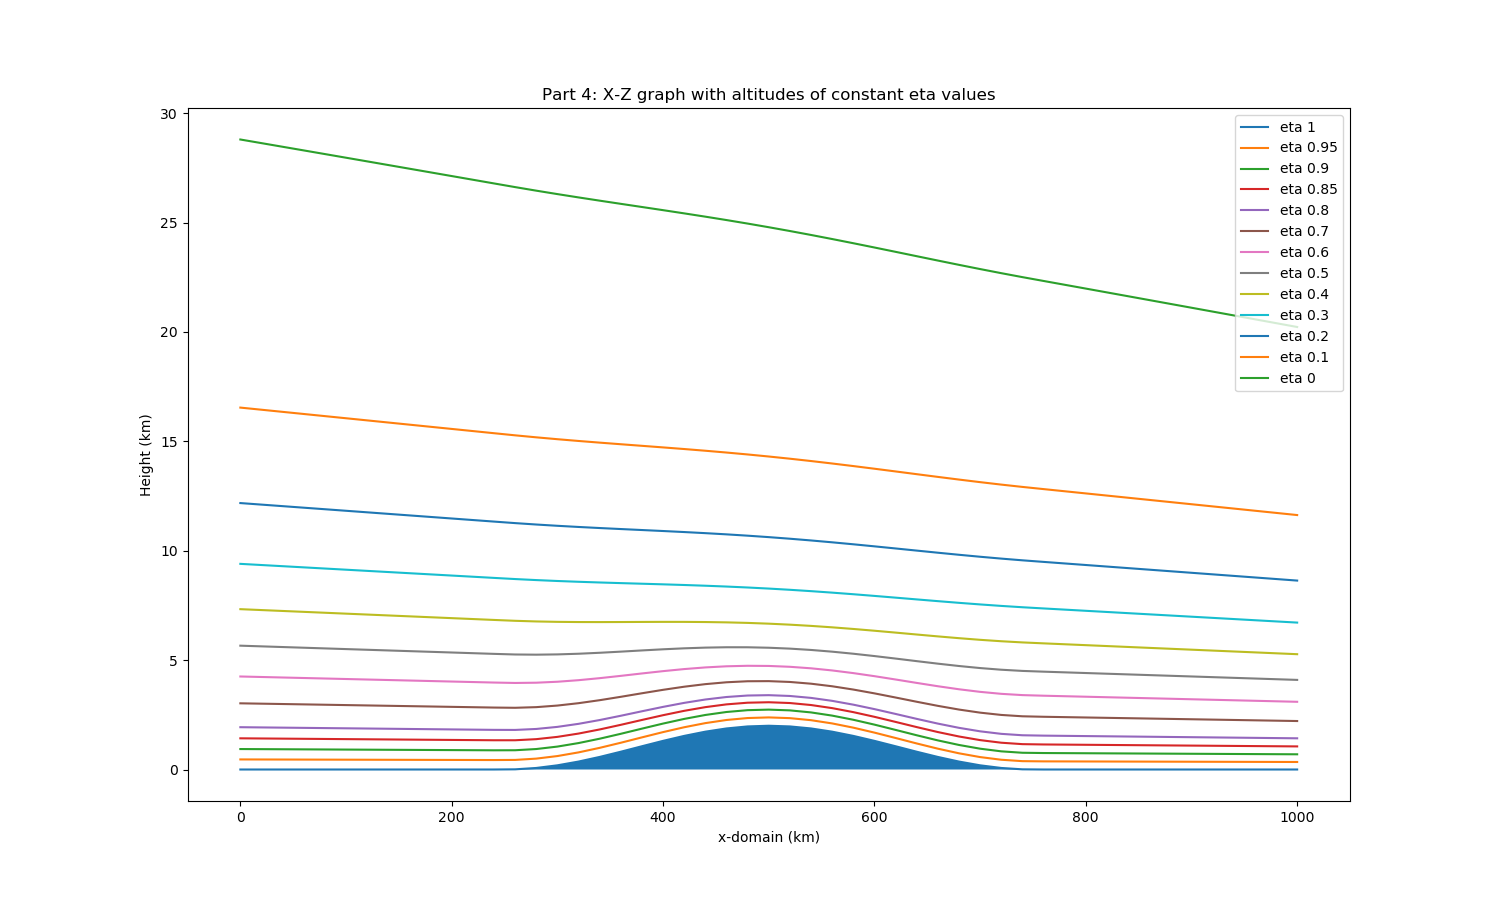
\includegraphics[width=\textwidth]{200120part4_plot.png}
    \caption{x-z plot of altitude for constant $ \eta $ with the ground shown by the shaded blue area.}
    \label{fig:mesh1}
\end{figure}


\newpage
\section*{Appendix 1 - Part 2 table}

\begin{longtable}{|l|l|l|l|}
\caption {Table to show surface pressure from two methods of interpolation} \\
    \hline
    \textbf{x (km)} & \textbf{z\_ground (km)} & \textbf{p\_sfc - hypsometric (kPa)} & \textbf{p\_sfc - interpolation (kPa)} \\ \hline
    \hline
    \endhead
    %
    0    & 0           & 95                         & 95                      \\ \hline
    20   & 0           & 95.2                       & 95.2                    \\ \hline
    40   & 0           & 95.4                       & 95.4                    \\ \hline
    60   & 0           & 95.6                       & 95.6                    \\ \hline
    80   & 0           & 95.8                       & 95.8                    \\ \hline
    100  & 0           & 96                         & 96                      \\ \hline
    120  & 0           & 96.2                       & 96.2                    \\ \hline
    140  & 0           & 96.4                       & 96.4                    \\ \hline
    160  & 0           & 96.6                       & 96.6                    \\ \hline
    180  & 0           & 96.8                       & 96.8                    \\ \hline
    200  & 0           & 97                         & 97                      \\ \hline
    220  & 0           & 97.2                       & 97.2                    \\ \hline
    240  & 0           & 97.4                       & 97.4                    \\ \hline
    260  & 0.007885618 & 97.50810262                & 97.51333864             \\ \hline
    280  & 0.070224374 & 96.978406                  & 97.02256781             \\ \hline
    300  & 0.190984253 & 95.76469456                & 95.87005972             \\ \hline
    320  & 0.362577482 & 93.96784119                & 94.12641853             \\ \hline
    340  & 0.574222245 & 91.73210462                & 91.90061997             \\ \hline
    360  & 0.812620145 & 89.228383                  & 89.3336945              \\ \hline
    380  & 1.062791791 & 86.63658367                & 86.6597553              \\ \hline
    400  & 1.309018004 & 84.13009567                & 84.1949776              \\ \hline
    420  & 1.535827512 & 81.86428518                & 81.89793306             \\ \hline
    440  & 1.728969063 & 79.96962152                & 79.92339943             \\ \hline
    460  & 1.876306885 & 78.54890208                & 78.40785686             \\ \hline
    480  & 1.968583214 & 77.67732657                & 77.46060852             \\ \hline
    500  & 2           & 77.40391856                & 77.15649385             \\ \hline
    520  & 1.968583214 & 77.75291945                & 77.53067618             \\ \hline
    540  & 1.876306885 & 78.72415134                & 78.57586287             \\ \hline
    560  & 1.728969063 & 80.29185473                & 80.24216717             \\ \hline
    580  & 1.535827512 & 82.40208868                & 82.43965784             \\ \hline
    600  & 1.309018004 & 84.9693994                 & 85.04347319             \\ \hline
    620  & 1.062791791 & 87.8740627                 & 87.90121321             \\ \hline
    640  & 0.812620145 & 90.96167338                & 91.08899022             \\ \hline
    660  & 0.574222245 & 94.04700425                & 94.25653988             \\ \hline
    680  & 0.362577482 & 96.92367341                & 97.12650249             \\ \hline
    700  & 0.190984253 & 99.38010269                & 99.51873736             \\ \hline
    720  & 0.070224374 & 101.2206071                & 101.280375              \\ \hline
    740  & 0.007885618 & 102.2886199                & 102.2959073             \\ \hline
    760  & 0           & 102.6                      & 102.6                   \\ \hline
    780  & 0           & 102.8                      & 102.8                   \\ \hline
    800  & 0           & 103                        & 103                     \\ \hline
    820  & 0           & 103.2                      & 103.2                   \\ \hline
    840  & 0           & 103.4                      & 103.4                   \\ \hline
    860  & 0           & 103.6                      & 103.6                   \\ \hline
    880  & 0           & 103.8                      & 103.8                   \\ \hline
    900  & 0           & 104                        & 104                     \\ \hline
    920  & 0           & 104.2                      & 104.2                   \\ \hline
    940  & 0           & 104.4                      & 104.4                   \\ \hline
    960  & 0           & 104.6                      & 104.6                   \\ \hline
    980  & 0           & 104.8                      & 104.8                   \\ \hline
    1000 & 0           & 105                        & 105                     \\ \hline
    \end{longtable}


    \newpage
\section*{Appendix 2 - Code}

See following pages.

\includepdf[page={1,2,3,4,5}]{HW1code.pdf}


\end{document}
  

